\chapter[Order and Disorder in Procrystalline Lattices]{Order and Disorder in \\ Procrystalline Lattices} 

\begin{chapterabstract}
Recent work has introduced the term ``procrystalline'' to define systems which lack translational symmetry but have an underlying high symmetry lattice, owing to a difference between the coordination numbers of the molecular units and the underlying lattice.
These materials are expected to lie between crystalline and amorphous phases.
The network properties of a range of these procrystals are investigated, encompassing a series of coordination environments.
Configurations are generated using a zero\--temperature \mc{} method, whilst simpler lattices are also considered analytically.
Procrystals are shown to be rare examples of systems with violate \lm{}'s law, whilst also displaying assortativities different to those calculated for amorphous materials.
Procrystalline lattices are therefore shown to have fundamentally different behaviour to traditional disordered and crystalline systems, indicative of the partial ordering of the underlying lattices.
\end{chapterabstract}

\section{The Procrystalline State}

Investigations into inorganic network\--forming materials have led to the introduction of the term ``procrystalline'' to refer to systems in which molecular building blocks lie on a regular array of lattice points, but directional interactions lead to overall correlated disorder \cite{Overy2016}.
As an introductory example, consider the procrystal in figure \ref{fig:prointroa}.
In this configuration the nodes form a square net, but each lattice site is occupied by a ``T'' shaped unit.
If the ends of these units are mutually attractive, they will orient to maximise favourable interactions.
The consequence of this is to introduce disorder into the ring structure.
This can be detected in the dual network, as in figure \ref{fig:prointrob}, which in this case can be viewed as a defective square net.
More strikingly, a system of percolating rings once again emerges, highlighted in figure \ref{fig:prointroc}, in analogue with networks from previous chapters. 

\begin{figure}[bt]
     \centering
     
     \begin{subfigure}[b]{0.3\textwidth}
         \centering
         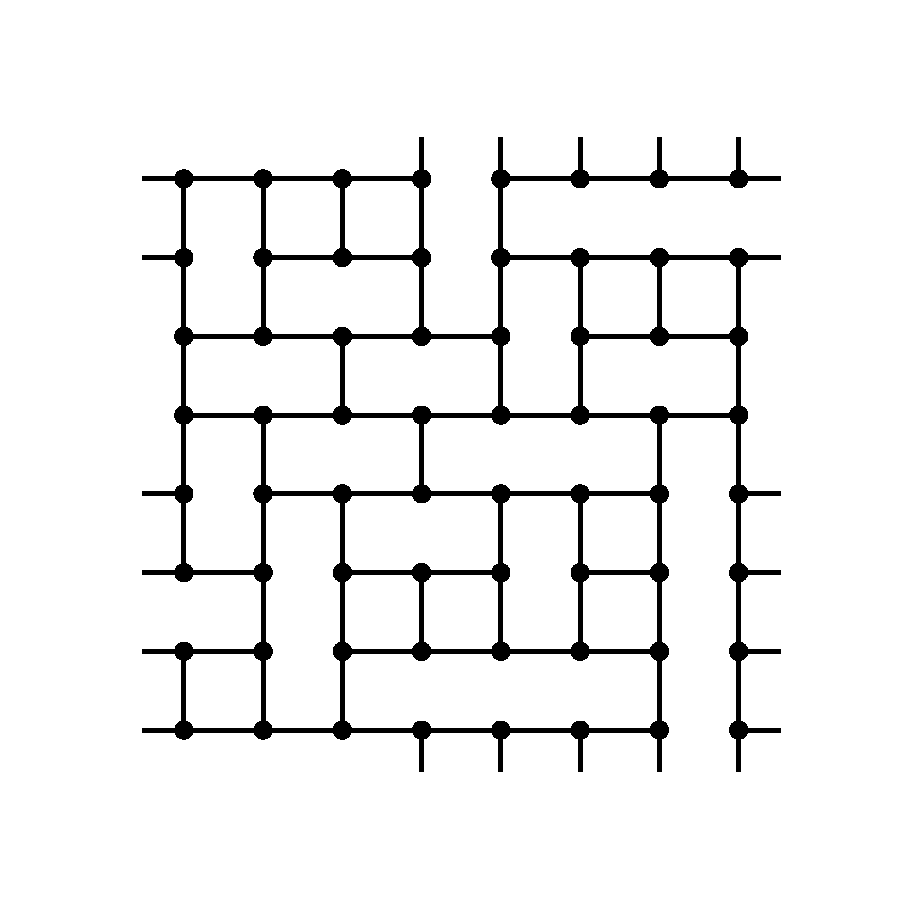
\includegraphics[width=\textwidth]{./figures/procrystals/pro_intro3.pdf}
         \caption{Procrystalline lattice}
         \label{fig:prointroa}
     \end{subfigure}
     \hfill
      \begin{subfigure}[b]{0.3\textwidth}
         \centering
         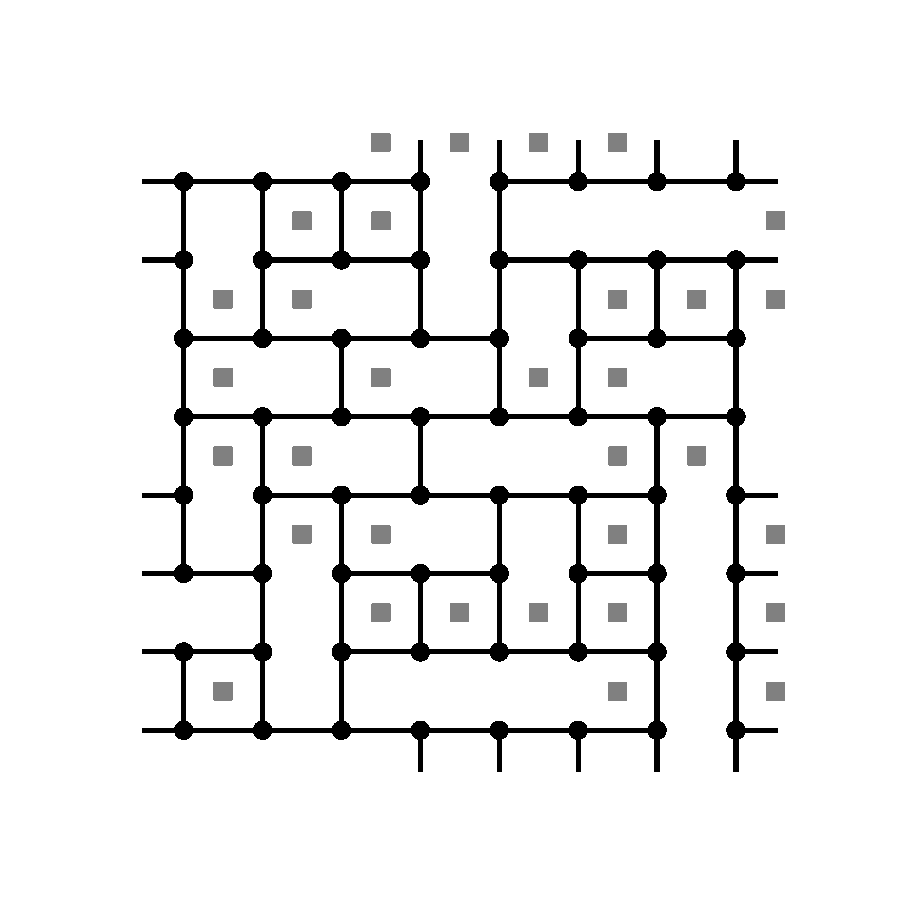
\includegraphics[width=\textwidth]{./figures/procrystals/pro_intro1.pdf}
         \caption{Overlay with dual}
         \label{fig:prointrob}
     \end{subfigure}
     \hfill
     \begin{subfigure}[b]{0.3\textwidth}
         \centering
         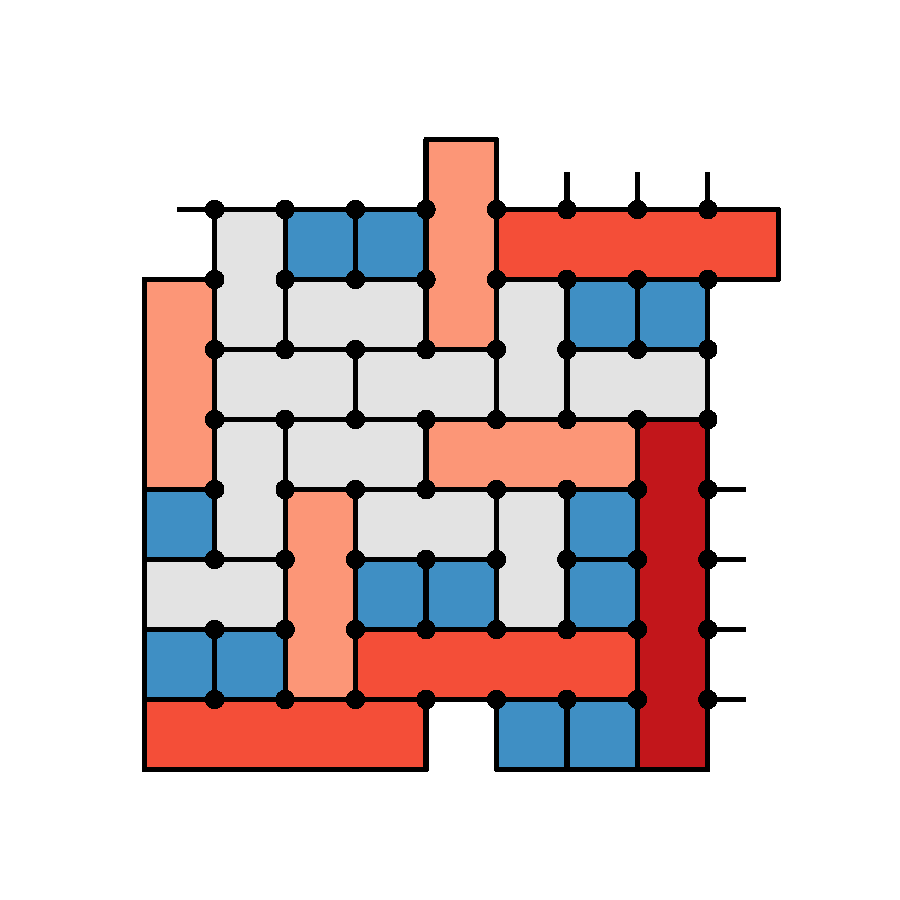
\includegraphics[width=\textwidth]{./figures/procrystals/pro_intro2.pdf}
         \caption{Ring Structure}
         \label{fig:prointroc}
     \end{subfigure}
     
     \caption{Example procrystalline lattice based on the square net. Panel (a) shows the lattice with each node representing a 3\--coordinate molecular unit. Panel (b) adds the nodes of the dual network, which form a defective square lattice. Panel (c) highlights the corresponding ring structure, coloured by ring size.}
     \label{fig:nprointro}
\end{figure}

The local environment around each node in a procrystal is therefore identical, leading them to appear crystalline in their atomic RDFs and structure factors. 
However, considering the network in its entirety with both nodes and links, it is clear an infinite procrystalline lattice has no unit cell.
As such procrystals can be considered to sit somewhere in between traditional crystals and the amorphous materials discussed in previous chapters.
This ``partial disordering'' is expected to be reflected in their structural and electronic properties.

Experimentally there are several systems which can be thought of as realisations of procrystals. 
These include self-assembled molecular monolayers, classical bond valence solids, mixed-anion perovskites, and order/disorder ferroelectrics \cite{Blunt2008,Anderson1973,Camp2012,Comes1968}.


